% Options for packages loaded elsewhere
\PassOptionsToPackage{unicode}{hyperref}
\PassOptionsToPackage{hyphens}{url}
\PassOptionsToPackage{dvipsnames,svgnames,x11names}{xcolor}
%
\documentclass[
  letterpaper,
  DIV=11,
  numbers=noendperiod]{scrartcl}

\usepackage{amsmath,amssymb}
\usepackage{iftex}
\ifPDFTeX
  \usepackage[T1]{fontenc}
  \usepackage[utf8]{inputenc}
  \usepackage{textcomp} % provide euro and other symbols
\else % if luatex or xetex
  \usepackage{unicode-math}
  \defaultfontfeatures{Scale=MatchLowercase}
  \defaultfontfeatures[\rmfamily]{Ligatures=TeX,Scale=1}
\fi
\usepackage{lmodern}
\ifPDFTeX\else  
    % xetex/luatex font selection
\fi
% Use upquote if available, for straight quotes in verbatim environments
\IfFileExists{upquote.sty}{\usepackage{upquote}}{}
\IfFileExists{microtype.sty}{% use microtype if available
  \usepackage[]{microtype}
  \UseMicrotypeSet[protrusion]{basicmath} % disable protrusion for tt fonts
}{}
\makeatletter
\@ifundefined{KOMAClassName}{% if non-KOMA class
  \IfFileExists{parskip.sty}{%
    \usepackage{parskip}
  }{% else
    \setlength{\parindent}{0pt}
    \setlength{\parskip}{6pt plus 2pt minus 1pt}}
}{% if KOMA class
  \KOMAoptions{parskip=half}}
\makeatother
\usepackage{xcolor}
\setlength{\emergencystretch}{3em} % prevent overfull lines
\setcounter{secnumdepth}{-\maxdimen} % remove section numbering
% Make \paragraph and \subparagraph free-standing
\ifx\paragraph\undefined\else
  \let\oldparagraph\paragraph
  \renewcommand{\paragraph}[1]{\oldparagraph{#1}\mbox{}}
\fi
\ifx\subparagraph\undefined\else
  \let\oldsubparagraph\subparagraph
  \renewcommand{\subparagraph}[1]{\oldsubparagraph{#1}\mbox{}}
\fi

\usepackage{color}
\usepackage{fancyvrb}
\newcommand{\VerbBar}{|}
\newcommand{\VERB}{\Verb[commandchars=\\\{\}]}
\DefineVerbatimEnvironment{Highlighting}{Verbatim}{commandchars=\\\{\}}
% Add ',fontsize=\small' for more characters per line
\usepackage{framed}
\definecolor{shadecolor}{RGB}{241,243,245}
\newenvironment{Shaded}{\begin{snugshade}}{\end{snugshade}}
\newcommand{\AlertTok}[1]{\textcolor[rgb]{0.68,0.00,0.00}{#1}}
\newcommand{\AnnotationTok}[1]{\textcolor[rgb]{0.37,0.37,0.37}{#1}}
\newcommand{\AttributeTok}[1]{\textcolor[rgb]{0.40,0.45,0.13}{#1}}
\newcommand{\BaseNTok}[1]{\textcolor[rgb]{0.68,0.00,0.00}{#1}}
\newcommand{\BuiltInTok}[1]{\textcolor[rgb]{0.00,0.23,0.31}{#1}}
\newcommand{\CharTok}[1]{\textcolor[rgb]{0.13,0.47,0.30}{#1}}
\newcommand{\CommentTok}[1]{\textcolor[rgb]{0.37,0.37,0.37}{#1}}
\newcommand{\CommentVarTok}[1]{\textcolor[rgb]{0.37,0.37,0.37}{\textit{#1}}}
\newcommand{\ConstantTok}[1]{\textcolor[rgb]{0.56,0.35,0.01}{#1}}
\newcommand{\ControlFlowTok}[1]{\textcolor[rgb]{0.00,0.23,0.31}{#1}}
\newcommand{\DataTypeTok}[1]{\textcolor[rgb]{0.68,0.00,0.00}{#1}}
\newcommand{\DecValTok}[1]{\textcolor[rgb]{0.68,0.00,0.00}{#1}}
\newcommand{\DocumentationTok}[1]{\textcolor[rgb]{0.37,0.37,0.37}{\textit{#1}}}
\newcommand{\ErrorTok}[1]{\textcolor[rgb]{0.68,0.00,0.00}{#1}}
\newcommand{\ExtensionTok}[1]{\textcolor[rgb]{0.00,0.23,0.31}{#1}}
\newcommand{\FloatTok}[1]{\textcolor[rgb]{0.68,0.00,0.00}{#1}}
\newcommand{\FunctionTok}[1]{\textcolor[rgb]{0.28,0.35,0.67}{#1}}
\newcommand{\ImportTok}[1]{\textcolor[rgb]{0.00,0.46,0.62}{#1}}
\newcommand{\InformationTok}[1]{\textcolor[rgb]{0.37,0.37,0.37}{#1}}
\newcommand{\KeywordTok}[1]{\textcolor[rgb]{0.00,0.23,0.31}{#1}}
\newcommand{\NormalTok}[1]{\textcolor[rgb]{0.00,0.23,0.31}{#1}}
\newcommand{\OperatorTok}[1]{\textcolor[rgb]{0.37,0.37,0.37}{#1}}
\newcommand{\OtherTok}[1]{\textcolor[rgb]{0.00,0.23,0.31}{#1}}
\newcommand{\PreprocessorTok}[1]{\textcolor[rgb]{0.68,0.00,0.00}{#1}}
\newcommand{\RegionMarkerTok}[1]{\textcolor[rgb]{0.00,0.23,0.31}{#1}}
\newcommand{\SpecialCharTok}[1]{\textcolor[rgb]{0.37,0.37,0.37}{#1}}
\newcommand{\SpecialStringTok}[1]{\textcolor[rgb]{0.13,0.47,0.30}{#1}}
\newcommand{\StringTok}[1]{\textcolor[rgb]{0.13,0.47,0.30}{#1}}
\newcommand{\VariableTok}[1]{\textcolor[rgb]{0.07,0.07,0.07}{#1}}
\newcommand{\VerbatimStringTok}[1]{\textcolor[rgb]{0.13,0.47,0.30}{#1}}
\newcommand{\WarningTok}[1]{\textcolor[rgb]{0.37,0.37,0.37}{\textit{#1}}}

\providecommand{\tightlist}{%
  \setlength{\itemsep}{0pt}\setlength{\parskip}{0pt}}\usepackage{longtable,booktabs,array}
\usepackage{calc} % for calculating minipage widths
% Correct order of tables after \paragraph or \subparagraph
\usepackage{etoolbox}
\makeatletter
\patchcmd\longtable{\par}{\if@noskipsec\mbox{}\fi\par}{}{}
\makeatother
% Allow footnotes in longtable head/foot
\IfFileExists{footnotehyper.sty}{\usepackage{footnotehyper}}{\usepackage{footnote}}
\makesavenoteenv{longtable}
\usepackage{graphicx}
\makeatletter
\def\maxwidth{\ifdim\Gin@nat@width>\linewidth\linewidth\else\Gin@nat@width\fi}
\def\maxheight{\ifdim\Gin@nat@height>\textheight\textheight\else\Gin@nat@height\fi}
\makeatother
% Scale images if necessary, so that they will not overflow the page
% margins by default, and it is still possible to overwrite the defaults
% using explicit options in \includegraphics[width, height, ...]{}
\setkeys{Gin}{width=\maxwidth,height=\maxheight,keepaspectratio}
% Set default figure placement to htbp
\makeatletter
\def\fps@figure{htbp}
\makeatother

\usepackage{booktabs}
\usepackage{longtable}
\usepackage{array}
\usepackage{multirow}
\usepackage{wrapfig}
\usepackage{float}
\usepackage{colortbl}
\usepackage{pdflscape}
\usepackage{tabu}
\usepackage{threeparttable}
\usepackage{threeparttablex}
\usepackage[normalem]{ulem}
\usepackage{makecell}
\usepackage{xcolor}
\KOMAoption{captions}{tableheading}
\makeatletter
\@ifpackageloaded{caption}{}{\usepackage{caption}}
\AtBeginDocument{%
\ifdefined\contentsname
  \renewcommand*\contentsname{Table of contents}
\else
  \newcommand\contentsname{Table of contents}
\fi
\ifdefined\listfigurename
  \renewcommand*\listfigurename{List of Figures}
\else
  \newcommand\listfigurename{List of Figures}
\fi
\ifdefined\listtablename
  \renewcommand*\listtablename{List of Tables}
\else
  \newcommand\listtablename{List of Tables}
\fi
\ifdefined\figurename
  \renewcommand*\figurename{Figure}
\else
  \newcommand\figurename{Figure}
\fi
\ifdefined\tablename
  \renewcommand*\tablename{Table}
\else
  \newcommand\tablename{Table}
\fi
}
\@ifpackageloaded{float}{}{\usepackage{float}}
\floatstyle{ruled}
\@ifundefined{c@chapter}{\newfloat{codelisting}{h}{lop}}{\newfloat{codelisting}{h}{lop}[chapter]}
\floatname{codelisting}{Listing}
\newcommand*\listoflistings{\listof{codelisting}{List of Listings}}
\makeatother
\makeatletter
\makeatother
\makeatletter
\@ifpackageloaded{caption}{}{\usepackage{caption}}
\@ifpackageloaded{subcaption}{}{\usepackage{subcaption}}
\makeatother
\ifLuaTeX
  \usepackage{selnolig}  % disable illegal ligatures
\fi
\usepackage{bookmark}

\IfFileExists{xurl.sty}{\usepackage{xurl}}{} % add URL line breaks if available
\urlstyle{same} % disable monospaced font for URLs
\hypersetup{
  pdftitle={Assignment2\_Data608\_Quarto},
  pdfauthor={Mubashira Qari},
  colorlinks=true,
  linkcolor={blue},
  filecolor={Maroon},
  citecolor={Blue},
  urlcolor={Blue},
  pdfcreator={LaTeX via pandoc}}

\title{Assignment2\_Data608\_Quarto}
\author{Mubashira Qari}
\date{}

\begin{document}
\maketitle

\subsection{Quarto}\label{quarto}

Quarto enables you to weave together content and executable code into a
finished document. To learn more about Quarto see
\url{https://quarto.org}.

The \texttt{echo:\ false} option disables the printing of code (only
output is displayed).

\subsubsection{Load Libraries}\label{load-libraries}

\begin{Shaded}
\begin{Highlighting}[]
\CommentTok{\#install.packages("tinytex")}
\CommentTok{\#tinytex::install\_tinytex()  \# Install TinyTeX (if not installed)}
\CommentTok{\#tinytex::tlmgr\_install("koma{-}script")  \# Install the missing KOMA{-}Script package}
\end{Highlighting}
\end{Shaded}

\begin{Shaded}
\begin{Highlighting}[]
\FunctionTok{library}\NormalTok{(tidyverse)}
\end{Highlighting}
\end{Shaded}

\begin{verbatim}
-- Attaching core tidyverse packages ------------------------ tidyverse 2.0.0 --
v dplyr     1.1.4     v readr     2.1.5
v forcats   1.0.0     v stringr   1.5.1
v ggplot2   3.5.1     v tibble    3.2.1
v lubridate 1.9.4     v tidyr     1.3.1
v purrr     1.0.2     
-- Conflicts ------------------------------------------ tidyverse_conflicts() --
x dplyr::filter() masks stats::filter()
x dplyr::lag()    masks stats::lag()
i Use the conflicted package (<http://conflicted.r-lib.org/>) to force all conflicts to become errors
\end{verbatim}

\begin{Shaded}
\begin{Highlighting}[]
\FunctionTok{library}\NormalTok{(readxl)}
\FunctionTok{library}\NormalTok{(ggplot2)}
\FunctionTok{library}\NormalTok{(dplyr)}
\FunctionTok{library}\NormalTok{(stringr)}
\FunctionTok{library}\NormalTok{(tools)}
\FunctionTok{library}\NormalTok{(stringdist)}
\end{Highlighting}
\end{Shaded}

\begin{verbatim}

Attaching package: 'stringdist'

The following object is masked from 'package:tidyr':

    extract
\end{verbatim}

\begin{Shaded}
\begin{Highlighting}[]
\FunctionTok{library}\NormalTok{(broom)}
\FunctionTok{library}\NormalTok{(gridExtra)}
\end{Highlighting}
\end{Shaded}

\begin{verbatim}

Attaching package: 'gridExtra'

The following object is masked from 'package:dplyr':

    combine
\end{verbatim}

\begin{Shaded}
\begin{Highlighting}[]
\FunctionTok{library}\NormalTok{(gclus)}
\end{Highlighting}
\end{Shaded}

\begin{verbatim}
Loading required package: cluster
\end{verbatim}

\begin{Shaded}
\begin{Highlighting}[]
\FunctionTok{library}\NormalTok{(car)}
\end{Highlighting}
\end{Shaded}

\begin{verbatim}
Loading required package: carData

Attaching package: 'car'

The following object is masked from 'package:dplyr':

    recode

The following object is masked from 'package:purrr':

    some
\end{verbatim}

\begin{Shaded}
\begin{Highlighting}[]
\FunctionTok{library}\NormalTok{(VGAM)}
\end{Highlighting}
\end{Shaded}

\begin{verbatim}
Loading required package: stats4
Loading required package: splines

Attaching package: 'VGAM'

The following object is masked from 'package:car':

    logit
\end{verbatim}

\begin{Shaded}
\begin{Highlighting}[]
\FunctionTok{library}\NormalTok{(MASS)}
\end{Highlighting}
\end{Shaded}

\begin{verbatim}

Attaching package: 'MASS'

The following object is masked from 'package:dplyr':

    select
\end{verbatim}

\begin{Shaded}
\begin{Highlighting}[]
\FunctionTok{library}\NormalTok{(rpart.plot)}
\end{Highlighting}
\end{Shaded}

\begin{verbatim}
Loading required package: rpart
\end{verbatim}

\begin{Shaded}
\begin{Highlighting}[]
\FunctionTok{library}\NormalTok{(ggfortify)}
\FunctionTok{library}\NormalTok{(gridExtra)}
\FunctionTok{library}\NormalTok{(forecast)}
\end{Highlighting}
\end{Shaded}

\begin{verbatim}
Registered S3 method overwritten by 'quantmod':
  method            from
  as.zoo.data.frame zoo 
Registered S3 methods overwritten by 'forecast':
  method                 from     
  autoplot.Arima         ggfortify
  autoplot.acf           ggfortify
  autoplot.ar            ggfortify
  autoplot.bats          ggfortify
  autoplot.decomposed.ts ggfortify
  autoplot.ets           ggfortify
  autoplot.forecast      ggfortify
  autoplot.stl           ggfortify
  autoplot.ts            ggfortify
  fitted.ar              ggfortify
  fortify.ts             ggfortify
  residuals.ar           ggfortify
\end{verbatim}

\begin{Shaded}
\begin{Highlighting}[]
\FunctionTok{library}\NormalTok{(fpp2)}
\end{Highlighting}
\end{Shaded}

\begin{verbatim}
-- Attaching packages ---------------------------------------------- fpp2 2.5 --
v fma       2.5     v expsmooth 2.3
-- Conflicts ------------------------------------------------- fpp2_conflicts --
x car::some() masks purrr::some()
\end{verbatim}

\begin{Shaded}
\begin{Highlighting}[]
\FunctionTok{library}\NormalTok{(fma)}
\FunctionTok{library}\NormalTok{(kableExtra)}
\end{Highlighting}
\end{Shaded}

\begin{verbatim}

Attaching package: 'kableExtra'

The following object is masked from 'package:dplyr':

    group_rows
\end{verbatim}

\begin{Shaded}
\begin{Highlighting}[]
\FunctionTok{library}\NormalTok{(e1071)}
\FunctionTok{library}\NormalTok{(mlbench)}
\FunctionTok{library}\NormalTok{(ggcorrplot)}
\FunctionTok{library}\NormalTok{(DataExplorer)}
\FunctionTok{library}\NormalTok{(timeDate)}
\end{Highlighting}
\end{Shaded}

\begin{verbatim}

Attaching package: 'timeDate'

The following objects are masked from 'package:e1071':

    kurtosis, skewness
\end{verbatim}

\begin{Shaded}
\begin{Highlighting}[]
\FunctionTok{library}\NormalTok{(caret)}
\end{Highlighting}
\end{Shaded}

\begin{verbatim}
Loading required package: lattice

Attaching package: 'caret'

The following object is masked from 'package:VGAM':

    predictors

The following object is masked from 'package:purrr':

    lift
\end{verbatim}

\begin{Shaded}
\begin{Highlighting}[]
\FunctionTok{library}\NormalTok{(GGally)}
\end{Highlighting}
\end{Shaded}

\begin{verbatim}
Registered S3 method overwritten by 'GGally':
  method from   
  +.gg   ggplot2

Attaching package: 'GGally'

The following object is masked from 'package:fma':

    pigs
\end{verbatim}

\begin{Shaded}
\begin{Highlighting}[]
\FunctionTok{library}\NormalTok{(corrplot)}
\end{Highlighting}
\end{Shaded}

\begin{verbatim}
corrplot 0.92 loaded
\end{verbatim}

\begin{Shaded}
\begin{Highlighting}[]
\FunctionTok{library}\NormalTok{(RColorBrewer)}
\FunctionTok{library}\NormalTok{(tibble)}
\FunctionTok{library}\NormalTok{(tidyr)}
\FunctionTok{library}\NormalTok{(reshape2)}
\end{Highlighting}
\end{Shaded}

\begin{verbatim}

Attaching package: 'reshape2'

The following object is masked from 'package:tidyr':

    smiths
\end{verbatim}

\begin{Shaded}
\begin{Highlighting}[]
\FunctionTok{library}\NormalTok{(mixtools)}
\end{Highlighting}
\end{Shaded}

\begin{verbatim}
mixtools package, version 2.0.0, Released 2022-12-04
This package is based upon work supported by the National Science Foundation under Grant No. SES-0518772 and the Chan Zuckerberg Initiative: Essential Open Source Software for Science (Grant No. 2020-255193).


Attaching package: 'mixtools'

The following object is masked from 'package:car':

    ellipse
\end{verbatim}

\begin{Shaded}
\begin{Highlighting}[]
\FunctionTok{library}\NormalTok{(skimr)}
\end{Highlighting}
\end{Shaded}

\subsubsection{Loading Datasets}\label{loading-datasets}

\begin{Shaded}
\begin{Highlighting}[]
\NormalTok{unemployment\_data }\OtherTok{\textless{}{-}} \FunctionTok{read.csv}\NormalTok{(}\StringTok{"https://raw.githubusercontent.com/uzmabb182/Data\_608/refs/heads/main/Week\_2/unemployment\_rate.csv"}\NormalTok{)}

\NormalTok{fed\_data }\OtherTok{\textless{}{-}} \FunctionTok{read.csv}\NormalTok{(}\StringTok{"https://raw.githubusercontent.com/uzmabb182/Data\_608/refs/heads/main/Week\_2/fed\_fund\_rate.csv"}\NormalTok{)}

\NormalTok{cpi\_data }\OtherTok{\textless{}{-}} \FunctionTok{read.csv}\NormalTok{(}\StringTok{"https://raw.githubusercontent.com/uzmabb182/Data\_608/refs/heads/main/Week\_2/consumer\_price\_index.csv"}\NormalTok{)}

\CommentTok{\#print(unemployment\_data)}
\CommentTok{\#print(fed\_data)}
\CommentTok{\#print(cpi\_data)}
\end{Highlighting}
\end{Shaded}

\subsubsection{Remove the HALF1 and HALF2
columns}\label{remove-the-half1-and-half2-columns}

\begin{Shaded}
\begin{Highlighting}[]
\NormalTok{cpi\_df }\OtherTok{\textless{}{-}}\NormalTok{ cpi\_data[, }\SpecialCharTok{!}\NormalTok{(}\FunctionTok{names}\NormalTok{(cpi\_data) }\SpecialCharTok{\%in\%} \FunctionTok{c}\NormalTok{(}\StringTok{"HALF1"}\NormalTok{, }\StringTok{"HALF2"}\NormalTok{))]}
\end{Highlighting}
\end{Shaded}

\subsubsection{\texorpdfstring{Convert from wide format to long format
using
\texttt{reshape()}}{Convert from wide format to long format using reshape()}}\label{convert-from-wide-format-to-long-format-using-reshape}

\begin{Shaded}
\begin{Highlighting}[]
\NormalTok{cpi\_long }\OtherTok{\textless{}{-}} \FunctionTok{reshape}\NormalTok{(cpi\_df, }
                    \AttributeTok{varying =} \FunctionTok{list}\NormalTok{(}\DecValTok{2}\SpecialCharTok{:}\FunctionTok{ncol}\NormalTok{(cpi\_df)),  }\CommentTok{\# All columns except "Year"}
                    \AttributeTok{v.names =} \StringTok{"CPI"}\NormalTok{,  }\CommentTok{\# New column name for CPI values}
                    \AttributeTok{timevar =} \StringTok{"Month"}\NormalTok{,  }\CommentTok{\# New column for Month names}
                    \AttributeTok{times =} \FunctionTok{names}\NormalTok{(cpi\_df)[}\DecValTok{2}\SpecialCharTok{:}\FunctionTok{ncol}\NormalTok{(cpi\_df)],  }\CommentTok{\# Month names from column names}
                    \AttributeTok{idvar =} \StringTok{"Year"}\NormalTok{,  }\CommentTok{\# Keep Year column as identifier}
                    \AttributeTok{direction =} \StringTok{"long"}\NormalTok{)}
\CommentTok{\#cpi\_long}
\end{Highlighting}
\end{Shaded}

\subsubsection{Saving as CSV}\label{saving-as-csv}

\begin{Shaded}
\begin{Highlighting}[]
\CommentTok{\# Define the file path with filename and extension}
\CommentTok{\#file\_path \textless{}{-} "C:/Users/Uzma/Downloads/new\_df.csv"}
\NormalTok{file\_path }\OtherTok{\textless{}{-}} \StringTok{"C:/Users/Uzma/CUNY{-}SPS{-}Assignments/Data\_608/output\_csv/processed\_interest\_rates.csv"}
\CommentTok{\# Write dataframe to CSV}
\FunctionTok{write.csv}\NormalTok{(cpi\_long, }\AttributeTok{file =}\NormalTok{ file\_path, }\AttributeTok{row.names =} \ConstantTok{FALSE}\NormalTok{)}

\CommentTok{\# Confirm that the file was saved}
\FunctionTok{print}\NormalTok{(}\StringTok{"File saved successfully!"}\NormalTok{)}
\end{Highlighting}
\end{Shaded}

\begin{verbatim}
[1] "File saved successfully!"
\end{verbatim}

\begin{Shaded}
\begin{Highlighting}[]
\CommentTok{\#cpi\_long}
\end{Highlighting}
\end{Shaded}

\subsubsection{Calculate percentage change and round to 2 decimal
places}\label{calculate-percentage-change-and-round-to-2-decimal-places}

\begin{Shaded}
\begin{Highlighting}[]
\NormalTok{cpi\_df }\OtherTok{\textless{}{-}}\NormalTok{ cpi\_long }\SpecialCharTok{\%\textgreater{}\%}
  \FunctionTok{group\_by}\NormalTok{(Month) }\SpecialCharTok{\%\textgreater{}\%}  \CommentTok{\# Group by month to ensure comparisons are within the same month}
  \FunctionTok{mutate}\NormalTok{(}\StringTok{\textasciigrave{}}\AttributeTok{inflation\_rate}\StringTok{\textasciigrave{}} \OtherTok{=} \FunctionTok{round}\NormalTok{(((CPI }\SpecialCharTok{{-}} \FunctionTok{lag}\NormalTok{(CPI)) }\SpecialCharTok{/} \FunctionTok{lag}\NormalTok{(CPI)) }\SpecialCharTok{*} \DecValTok{100}\NormalTok{, }\DecValTok{2}\NormalTok{)) }\SpecialCharTok{\%\textgreater{}\%}
  \FunctionTok{ungroup}\NormalTok{()}

\CommentTok{\#cpi\_df}
\end{Highlighting}
\end{Shaded}

\subsubsection{Create a new column `Status' based on
`inflation\_rate'}\label{create-a-new-column-status-based-on-inflation_rate}

\begin{Shaded}
\begin{Highlighting}[]
\NormalTok{cpi\_df }\OtherTok{\textless{}{-}}\NormalTok{ cpi\_df }\SpecialCharTok{\%\textgreater{}\%}
  \FunctionTok{mutate}\NormalTok{(}\AttributeTok{inflation\_criteria =} \FunctionTok{ifelse}\NormalTok{(inflation\_rate }\SpecialCharTok{\textgreater{}} \DecValTok{2}\NormalTok{, }\StringTok{"Not Achieved"}\NormalTok{, }\StringTok{"Achieved"}\NormalTok{))}

\CommentTok{\#cpi\_df}
\end{Highlighting}
\end{Shaded}

\subsubsection{Remove rows where Year is
1999}\label{remove-rows-where-year-is-1999}

\begin{Shaded}
\begin{Highlighting}[]
\NormalTok{cpi\_df }\OtherTok{\textless{}{-}}\NormalTok{ cpi\_df }\SpecialCharTok{\%\textgreater{}\%}
  \FunctionTok{filter}\NormalTok{(Year }\SpecialCharTok{!=} \DecValTok{1999}\NormalTok{)  }\CommentTok{\# Keep only rows where Year is NOT 1999}

\CommentTok{\#cpi\_df}
\end{Highlighting}
\end{Shaded}

\subsubsection{Saving as CSV}\label{saving-as-csv-1}

\begin{Shaded}
\begin{Highlighting}[]
\CommentTok{\# Define the file path with filename and extension}
\CommentTok{\#file\_path \textless{}{-} "C:/Users/Uzma/Downloads/new\_df.csv"}
\NormalTok{file\_path }\OtherTok{\textless{}{-}} \StringTok{"C:/Users/Uzma/CUNY{-}SPS{-}Assignments/Data\_608/output\_csv/inflation\_rates.csv"}
\CommentTok{\# Write dataframe to CSV}
\FunctionTok{write.csv}\NormalTok{(cpi\_df, }\AttributeTok{file =}\NormalTok{ file\_path, }\AttributeTok{row.names =} \ConstantTok{FALSE}\NormalTok{)}

\CommentTok{\# Confirm that the file was saved}
\FunctionTok{print}\NormalTok{(}\StringTok{"File saved successfully!"}\NormalTok{)}
\end{Highlighting}
\end{Shaded}

\begin{verbatim}
[1] "File saved successfully!"
\end{verbatim}

\begin{Shaded}
\begin{Highlighting}[]
\CommentTok{\#cpi\_df}
\end{Highlighting}
\end{Shaded}

\subsubsection{Preparing FED Dataset}\label{preparing-fed-dataset}

\begin{Shaded}
\begin{Highlighting}[]
\CommentTok{\#fed\_data}
\end{Highlighting}
\end{Shaded}

\subsubsection{Convert ``observation\_date'' to a Date
format}\label{convert-observation_date-to-a-date-format}

\begin{Shaded}
\begin{Highlighting}[]
\NormalTok{fed\_data }\OtherTok{\textless{}{-}}\NormalTok{ fed\_data }\SpecialCharTok{\%\textgreater{}\%}
  \FunctionTok{mutate}\NormalTok{(}\AttributeTok{observation\_date =} \FunctionTok{mdy}\NormalTok{(observation\_date))  }\CommentTok{\# Converts MM/DD/YYYY format to Date type}

\NormalTok{fed\_df }\OtherTok{\textless{}{-}}\NormalTok{ fed\_data}
\CommentTok{\#fed\_df}
\end{Highlighting}
\end{Shaded}

\subsubsection{Extract Year and Month}\label{extract-year-and-month}

\begin{Shaded}
\begin{Highlighting}[]
\NormalTok{fed\_df }\OtherTok{\textless{}{-}}\NormalTok{ fed\_df }\SpecialCharTok{\%\textgreater{}\%}
  \FunctionTok{mutate}\NormalTok{(}\AttributeTok{Year =} \FunctionTok{year}\NormalTok{(observation\_date),}
         \AttributeTok{Month =} \FunctionTok{month}\NormalTok{(observation\_date, }\AttributeTok{label =} \ConstantTok{TRUE}\NormalTok{, }\AttributeTok{abbr =} \ConstantTok{TRUE}\NormalTok{))  }\CommentTok{\# Extract month name (Jan, Feb, etc.)}

\CommentTok{\#fed\_df}
\end{Highlighting}
\end{Shaded}

\subsubsection{Saving as CSV}\label{saving-as-csv-2}

\begin{Shaded}
\begin{Highlighting}[]
\CommentTok{\# Define the file path with filename and extension}
\CommentTok{\#file\_path \textless{}{-} "C:/Users/Uzma/Downloads/new\_df.csv"}
\NormalTok{file\_path }\OtherTok{\textless{}{-}} \StringTok{"C:/Users/Uzma/CUNY{-}SPS{-}Assignments/Data\_608/output\_csv/fed\_rates.csv"}
\CommentTok{\# Write dataframe to CSV}
\FunctionTok{write.csv}\NormalTok{(fed\_df, }\AttributeTok{file =}\NormalTok{ file\_path, }\AttributeTok{row.names =} \ConstantTok{FALSE}\NormalTok{)}

\CommentTok{\# Confirm that the file was saved}
\CommentTok{\#print("File saved successfully!")}
\end{Highlighting}
\end{Shaded}

\subsubsection{Creating Dataframe for Unemployment Rate
dataset}\label{creating-dataframe-for-unemployment-rate-dataset}

\begin{Shaded}
\begin{Highlighting}[]
\NormalTok{unemp\_df }\OtherTok{\textless{}{-}}\NormalTok{ unemployment\_data}

\CommentTok{\#unemp\_df}
\end{Highlighting}
\end{Shaded}

\subsubsection{Extract the Month from the Label
column}\label{extract-the-month-from-the-label-column}

\begin{Shaded}
\begin{Highlighting}[]
\NormalTok{unemp\_df }\OtherTok{\textless{}{-}}\NormalTok{ unemp\_df }\SpecialCharTok{\%\textgreater{}\%}
  \FunctionTok{mutate}\NormalTok{(}\AttributeTok{Month =} \FunctionTok{word}\NormalTok{(Label, }\DecValTok{2}\NormalTok{))  }\CommentTok{\# Extract the second word (month name) from "1999 Jan"}

\CommentTok{\#unemp\_df}
\end{Highlighting}
\end{Shaded}

\subsubsection{Arrange dataset in chronological
order}\label{arrange-dataset-in-chronological-order}

\begin{Shaded}
\begin{Highlighting}[]
\NormalTok{unemp\_df }\OtherTok{\textless{}{-}}\NormalTok{ unemp\_df }\SpecialCharTok{\%\textgreater{}\%}
  \FunctionTok{arrange}\NormalTok{(Year, Month, unemployment\_rate)}

\CommentTok{\#unemp\_df}
\end{Highlighting}
\end{Shaded}

\subsubsection{Create a new column `Status' based on
`unemployment\_rate'}\label{create-a-new-column-status-based-on-unemployment_rate}

\begin{Shaded}
\begin{Highlighting}[]
\NormalTok{unemp\_df }\OtherTok{\textless{}{-}}\NormalTok{ unemp\_df }\SpecialCharTok{\%\textgreater{}\%}
  \FunctionTok{mutate}\NormalTok{(}\AttributeTok{unemp\_criteria =} \FunctionTok{ifelse}\NormalTok{(unemployment\_rate }\SpecialCharTok{\textgreater{}} \DecValTok{6}\NormalTok{, }\StringTok{"Not Achieved"}\NormalTok{, }\StringTok{"Achieved"}\NormalTok{))}

\CommentTok{\#unemp\_df}
\end{Highlighting}
\end{Shaded}

\subsubsection{Saving as CSV}\label{saving-as-csv-3}

\begin{Shaded}
\begin{Highlighting}[]
\CommentTok{\# Define the file path with filename and extension}
\CommentTok{\#file\_path \textless{}{-} "C:/Users/Uzma/Downloads/new\_df.csv"}
\NormalTok{file\_path }\OtherTok{\textless{}{-}} \StringTok{"C:/Users/Uzma/CUNY{-}SPS{-}Assignments/Data\_608/output\_csv/unemp\_rates.csv"}
\CommentTok{\# Write dataframe to CSV}
\FunctionTok{write.csv}\NormalTok{(unemp\_df, }\AttributeTok{file =}\NormalTok{ file\_path, }\AttributeTok{row.names =} \ConstantTok{FALSE}\NormalTok{)}

\CommentTok{\# Confirm that the file was saved}
\CommentTok{\#print("File saved successfully!")}
\end{Highlighting}
\end{Shaded}

\subsubsection{Visualizing FED's Mandate
Fulfillment}\label{visualizing-feds-mandate-fulfillment}

The Federal Reserve (FED) has a dual mandate from Congress:

Stable Prices (Low Inflation) → Inflation rate around 2\%

Maximum Employment (Low Unemployment) → Low unemployment
(\textasciitilde5\% or lower)

\subsubsection{Load Libraries}\label{load-libraries-1}

\begin{Shaded}
\begin{Highlighting}[]
\FunctionTok{library}\NormalTok{(ggplot2)  }
\FunctionTok{library}\NormalTok{(dplyr)     }
\FunctionTok{library}\NormalTok{(readr)     }
\FunctionTok{library}\NormalTok{(scales)    }
\end{Highlighting}
\end{Shaded}

\begin{verbatim}
Warning: package 'scales' was built under R version 4.3.3
\end{verbatim}

\begin{verbatim}

Attaching package: 'scales'
\end{verbatim}

\begin{verbatim}
The following object is masked from 'package:purrr':

    discard
\end{verbatim}

\begin{verbatim}
The following object is masked from 'package:readr':

    col_factor
\end{verbatim}

\subsubsection{Remove Year 1999}\label{remove-year-1999}

\begin{Shaded}
\begin{Highlighting}[]
\NormalTok{unemp\_df }\OtherTok{\textless{}{-}}\NormalTok{ unemp\_df }\SpecialCharTok{\%\textgreater{}\%} \FunctionTok{filter}\NormalTok{(Year }\SpecialCharTok{!=} \DecValTok{1999}\NormalTok{)}
\NormalTok{cpi\_df }\OtherTok{\textless{}{-}}\NormalTok{ cpi\_df }\SpecialCharTok{\%\textgreater{}\%} \FunctionTok{filter}\NormalTok{(Year }\SpecialCharTok{!=} \DecValTok{1999}\NormalTok{)}
\NormalTok{fed\_df }\OtherTok{\textless{}{-}}\NormalTok{ fed\_df }\SpecialCharTok{\%\textgreater{}\%} \FunctionTok{filter}\NormalTok{(Year }\SpecialCharTok{!=} \DecValTok{1999}\NormalTok{)}
\end{Highlighting}
\end{Shaded}

\subsubsection{Data Preparation: Merge All Three
Datasets}\label{data-preparation-merge-all-three-datasets}

\begin{Shaded}
\begin{Highlighting}[]
\NormalTok{merged\_df }\OtherTok{\textless{}{-}}\NormalTok{ unemp\_df }\SpecialCharTok{\%\textgreater{}\%}
  \FunctionTok{inner\_join}\NormalTok{(cpi\_df, }\AttributeTok{by =} \FunctionTok{c}\NormalTok{(}\StringTok{"Year"}\NormalTok{, }\StringTok{"Month"}\NormalTok{)) }\SpecialCharTok{\%\textgreater{}\%}
  \FunctionTok{inner\_join}\NormalTok{(fed\_df, }\AttributeTok{by =} \FunctionTok{c}\NormalTok{(}\StringTok{"Year"}\NormalTok{, }\StringTok{"Month"}\NormalTok{))}

\CommentTok{\#merged\_df}
\end{Highlighting}
\end{Shaded}

\subsubsection{Creating a Status Field}\label{creating-a-status-field}

\begin{Shaded}
\begin{Highlighting}[]
\NormalTok{merged\_df }\OtherTok{\textless{}{-}}\NormalTok{ merged\_df }\SpecialCharTok{\%\textgreater{}\%}
  \FunctionTok{mutate}\NormalTok{(}
    \AttributeTok{status =} \FunctionTok{case\_when}\NormalTok{(}
\NormalTok{      unemp\_criteria }\SpecialCharTok{==} \StringTok{"Achieved"} \SpecialCharTok{\&}\NormalTok{ inflation\_criteria }\SpecialCharTok{==} \StringTok{"Achieved"} \SpecialCharTok{\textasciitilde{}} \StringTok{"Yes"}\NormalTok{,}
\NormalTok{      unemp\_criteria }\SpecialCharTok{==} \StringTok{"Not Achieved"} \SpecialCharTok{\&}\NormalTok{ inflation\_criteria }\SpecialCharTok{==} \StringTok{"Not Achieved"} \SpecialCharTok{\textasciitilde{}} \StringTok{"No"}\NormalTok{,}
      \ConstantTok{TRUE} \SpecialCharTok{\textasciitilde{}} \StringTok{"Partial Achieved"}
\NormalTok{    )}
\NormalTok{  )}

\CommentTok{\#merged\_df}
\end{Highlighting}
\end{Shaded}

\subsubsection{Saving as CSV}\label{saving-as-csv-4}

\begin{Shaded}
\begin{Highlighting}[]
\CommentTok{\# Define the file path with filename and extension}
\CommentTok{\#file\_path \textless{}{-} "C:/Users/Uzma/Downloads/new\_df.csv"}
\NormalTok{file\_path }\OtherTok{\textless{}{-}} \StringTok{"C:/Users/Uzma/CUNY{-}SPS{-}Assignments/Data\_608/output\_csv/merged\_data.csv"}
\CommentTok{\# Write dataframe to CSV}
\CommentTok{\#write.csv(merged\_df, file = file\_path, row.names = FALSE)}

\CommentTok{\# Confirm that the file was saved}
\CommentTok{\#print("File saved successfully!")}
\end{Highlighting}
\end{Shaded}

\subsubsection{Visualization: Has the FED Fulfilled its
Mandate?}\label{visualization-has-the-fed-fulfilled-its-mandate}

\subsubsection{Unemployment, Inflation \& Fed Funds Rate
Trend}\label{unemployment-inflation-fed-funds-rate-trend}

This line chart shows how the unemployment rate, inflation rate, and Fed
Funds rate have changed over time.

\begin{Shaded}
\begin{Highlighting}[]
\CommentTok{\# Create a combined plot with dual y{-}axes}
\FunctionTok{ggplot}\NormalTok{(merged\_df, }\FunctionTok{aes}\NormalTok{(}\AttributeTok{x =} \FunctionTok{as.Date}\NormalTok{(}\FunctionTok{paste}\NormalTok{(Year, Month, }\StringTok{"1"}\NormalTok{, }\AttributeTok{sep =} \StringTok{"{-}"}\NormalTok{), }\StringTok{"\%Y{-}\%b{-}\%d"}\NormalTok{))) }\SpecialCharTok{+}
  \FunctionTok{geom\_line}\NormalTok{(}\FunctionTok{aes}\NormalTok{(}\AttributeTok{y =}\NormalTok{ unemployment\_rate, }\AttributeTok{color =} \StringTok{"Unemployment Rate"}\NormalTok{), }\AttributeTok{size =} \FloatTok{1.2}\NormalTok{) }\SpecialCharTok{+}
  \FunctionTok{geom\_line}\NormalTok{(}\FunctionTok{aes}\NormalTok{(}\AttributeTok{y =}\NormalTok{ inflation\_rate, }\AttributeTok{color =} \StringTok{"Inflation Rate"}\NormalTok{), }\AttributeTok{size =} \FloatTok{1.2}\NormalTok{) }\SpecialCharTok{+}
  \FunctionTok{geom\_line}\NormalTok{(}\FunctionTok{aes}\NormalTok{(}\AttributeTok{y =}\NormalTok{ fed\_fund\_rate, }\AttributeTok{color =} \StringTok{"Fed Funds Rate"}\NormalTok{), }\AttributeTok{size =} \FloatTok{1.2}\NormalTok{, }\AttributeTok{linetype =} \StringTok{"dashed"}\NormalTok{) }\SpecialCharTok{+}
  \FunctionTok{scale\_y\_continuous}\NormalTok{(}\AttributeTok{sec.axis =} \FunctionTok{sec\_axis}\NormalTok{(}\SpecialCharTok{\textasciitilde{}}\NormalTok{., }\AttributeTok{name =} \StringTok{"Fed Funds Rate (\%)"}\NormalTok{)) }\SpecialCharTok{+}
  \FunctionTok{labs}\NormalTok{(}\AttributeTok{title =} \StringTok{"Unemployment \& Inflation vs. Fed Funds Rate"}\NormalTok{,}
       \AttributeTok{x =} \StringTok{"Year"}\NormalTok{, }
       \AttributeTok{y =} \StringTok{"Unemployment \& Inflation (\%)"}\NormalTok{,}
       \AttributeTok{color =} \StringTok{"Legend"}\NormalTok{) }\SpecialCharTok{+}
  \FunctionTok{theme\_minimal}\NormalTok{()}
\end{Highlighting}
\end{Shaded}

\begin{verbatim}
Warning: Using `size` aesthetic for lines was deprecated in ggplot2 3.4.0.
i Please use `linewidth` instead.
\end{verbatim}

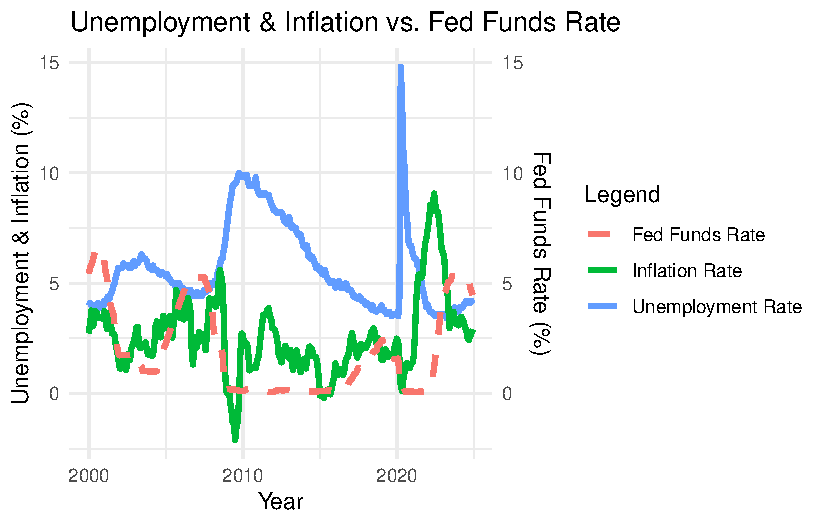
\includegraphics{Assignment2_Data608_Quarto_files/figure-pdf/unnamed-chunk-25-1.pdf}

\subsubsection{The Federal Reserve System has been given a dual mandate
of pursuing the economic goals of maximum employment and price stability
with a inflation rate of 2\% over time and unemployment rate between 4\%
and 6\% over
time}\label{the-federal-reserve-system-has-been-given-a-dual-mandate-of-pursuing-the-economic-goals-of-maximum-employment-and-price-stability-with-a-inflation-rate-of-2-over-time-and-unemployment-rate-between-4-and-6-over-time}

\subsubsection{``Has the FED been able to fulfill the mandate given to
it by
Congress?''}\label{has-the-fed-been-able-to-fulfill-the-mandate-given-to-it-by-congress}

\subsubsection{Unemployment Rate Over
Time}\label{unemployment-rate-over-time}

\begin{Shaded}
\begin{Highlighting}[]
\FunctionTok{ggplot}\NormalTok{(merged\_df, }\FunctionTok{aes}\NormalTok{(}\AttributeTok{x =} \FunctionTok{as.Date}\NormalTok{(}\FunctionTok{paste}\NormalTok{(Year, Month, }\StringTok{"1"}\NormalTok{, }\AttributeTok{sep =} \StringTok{"{-}"}\NormalTok{), }\StringTok{"\%Y{-}\%b{-}\%d"}\NormalTok{), }\AttributeTok{y =}\NormalTok{ unemployment\_rate)) }\SpecialCharTok{+}
  \FunctionTok{geom\_line}\NormalTok{(}\AttributeTok{color =} \StringTok{"blue"}\NormalTok{, }\AttributeTok{size =} \FloatTok{1.2}\NormalTok{) }\SpecialCharTok{+}
  \FunctionTok{geom\_hline}\NormalTok{(}\AttributeTok{yintercept =} \DecValTok{6}\NormalTok{, }\AttributeTok{linetype =} \StringTok{"dashed"}\NormalTok{, }\AttributeTok{color =} \StringTok{"red"}\NormalTok{) }\SpecialCharTok{+}
  \FunctionTok{labs}\NormalTok{(}\AttributeTok{title =} \StringTok{"Unemployment Rate Over Time"}\NormalTok{,}
       \AttributeTok{x =} \StringTok{"Year"}\NormalTok{, }
       \AttributeTok{y =} \StringTok{"Unemployment Rate (\%)"}\NormalTok{) }\SpecialCharTok{+}
  \FunctionTok{theme\_minimal}\NormalTok{()}
\end{Highlighting}
\end{Shaded}

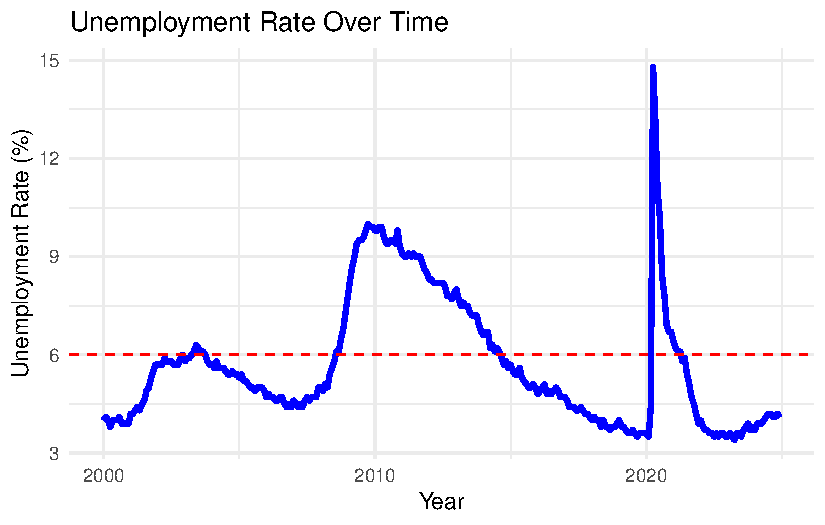
\includegraphics{Assignment2_Data608_Quarto_files/figure-pdf/unnamed-chunk-26-1.pdf}

Interpretation:

A dashed red line at 6\% shows the employment mandate If unemployment is
below 6\%, Fed is meeting its employment goal

\subsubsection{Inflation Rate Over Time}\label{inflation-rate-over-time}

\begin{Shaded}
\begin{Highlighting}[]
\FunctionTok{ggplot}\NormalTok{(merged\_df, }\FunctionTok{aes}\NormalTok{(}\AttributeTok{x =} \FunctionTok{as.Date}\NormalTok{(}\FunctionTok{paste}\NormalTok{(Year, Month, }\StringTok{"1"}\NormalTok{, }\AttributeTok{sep =} \StringTok{"{-}"}\NormalTok{), }\StringTok{"\%Y{-}\%b{-}\%d"}\NormalTok{), }\AttributeTok{y =}\NormalTok{ inflation\_rate)) }\SpecialCharTok{+}
  \FunctionTok{geom\_line}\NormalTok{(}\AttributeTok{color =} \StringTok{"green"}\NormalTok{, }\AttributeTok{size =} \FloatTok{1.2}\NormalTok{) }\SpecialCharTok{+}
  \FunctionTok{geom\_hline}\NormalTok{(}\AttributeTok{yintercept =} \DecValTok{2}\NormalTok{, }\AttributeTok{linetype =} \StringTok{"dashed"}\NormalTok{, }\AttributeTok{color =} \StringTok{"red"}\NormalTok{) }\SpecialCharTok{+}
  \FunctionTok{labs}\NormalTok{(}\AttributeTok{title =} \StringTok{"Inflation Rate Over Time"}\NormalTok{,}
       \AttributeTok{x =} \StringTok{"Year"}\NormalTok{, }
       \AttributeTok{y =} \StringTok{"Inflation Rate (\%)"}\NormalTok{) }\SpecialCharTok{+}
  \FunctionTok{theme\_minimal}\NormalTok{()}
\end{Highlighting}
\end{Shaded}

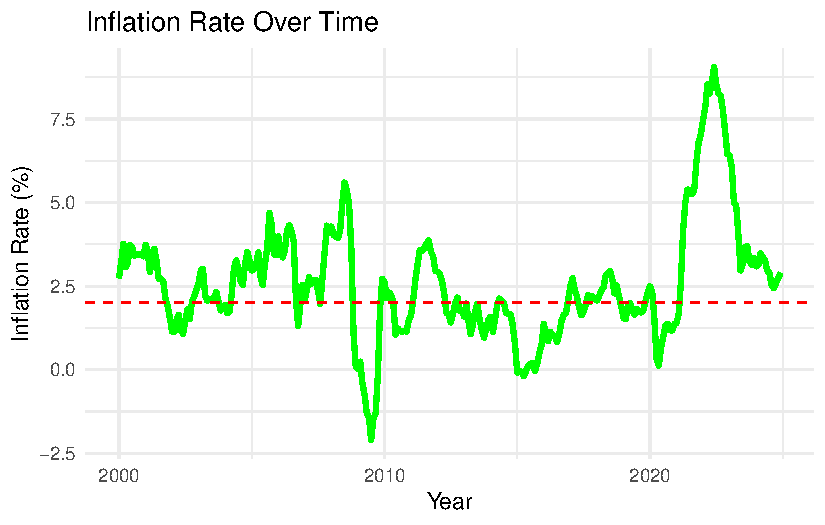
\includegraphics{Assignment2_Data608_Quarto_files/figure-pdf/unnamed-chunk-27-1.pdf}

Interpretation:

A dashed red line at 2\% shows the price stability mandate If inflation
stays near 2\%, Fed is achieving price stability

To evaluate whether the Federal Reserve (FED) has met its unemployment
mandate, we need to visualize unemployment trends over time and compare
them with the ``Achieved'' vs.~``Not Achieved'' status.

\begin{Shaded}
\begin{Highlighting}[]
\CommentTok{\# Convert Month to numeric and create Date column}
\NormalTok{unemp\_df }\OtherTok{\textless{}{-}}\NormalTok{ unemp\_df }\SpecialCharTok{\%\textgreater{}\%}
  \FunctionTok{mutate}\NormalTok{(}
    \AttributeTok{Month =} \FunctionTok{match}\NormalTok{(Month, month.abb),  }\CommentTok{\# Convert "Jan" {-}\textgreater{} 1, "Feb" {-}\textgreater{} 2}
    \AttributeTok{Date =} \FunctionTok{as.Date}\NormalTok{(}\FunctionTok{paste}\NormalTok{(Year, Month, }\StringTok{"1"}\NormalTok{, }\AttributeTok{sep =} \StringTok{"{-}"}\NormalTok{), }\AttributeTok{format =} \StringTok{"\%Y{-}\%m{-}\%d"}\NormalTok{),}
    \AttributeTok{unemployment\_rate =} \FunctionTok{as.numeric}\NormalTok{(unemployment\_rate)  }\CommentTok{\# Ensure numeric}
\NormalTok{  )}
\end{Highlighting}
\end{Shaded}

\begin{Shaded}
\begin{Highlighting}[]
\FunctionTok{ggplot}\NormalTok{(cpi\_df, }\FunctionTok{aes}\NormalTok{(}\AttributeTok{x =} \FunctionTok{factor}\NormalTok{(Year), }\AttributeTok{fill =}\NormalTok{ inflation\_criteria)) }\SpecialCharTok{+}
  \FunctionTok{geom\_bar}\NormalTok{(}\AttributeTok{position =} \StringTok{"stack"}\NormalTok{) }\SpecialCharTok{+}  
  \FunctionTok{scale\_fill\_manual}\NormalTok{(}\AttributeTok{values =} \FunctionTok{c}\NormalTok{(}\StringTok{"Achieved"} \OtherTok{=} \StringTok{"green"}\NormalTok{, }\StringTok{"Not Achieved"} \OtherTok{=} \StringTok{"orange"}\NormalTok{)) }\SpecialCharTok{+}
  \FunctionTok{scale\_y\_continuous}\NormalTok{(}\AttributeTok{breaks =} \FunctionTok{seq}\NormalTok{(}\DecValTok{0}\NormalTok{, }\DecValTok{12}\NormalTok{, }\AttributeTok{by =} \DecValTok{1}\NormalTok{)) }\SpecialCharTok{+}  \CommentTok{\# Force whole numbers for months}
  \FunctionTok{labs}\NormalTok{(}\AttributeTok{title =} \StringTok{"Inflation Mandate Achievement Over the Years"}\NormalTok{,}
       \AttributeTok{x =} \StringTok{"Year"}\NormalTok{,}
       \AttributeTok{y =} \StringTok{"Number of Months"}\NormalTok{,}
       \AttributeTok{fill =} \StringTok{"Mandate Status"}\NormalTok{) }\SpecialCharTok{+}
  \FunctionTok{theme\_minimal}\NormalTok{() }\SpecialCharTok{+}
  \FunctionTok{theme}\NormalTok{(}\AttributeTok{axis.text.x =} \FunctionTok{element\_text}\NormalTok{(}\AttributeTok{angle =} \DecValTok{45}\NormalTok{, }\AttributeTok{hjust =} \DecValTok{1}\NormalTok{))  }\CommentTok{\# Rotate x{-}axis labels for readability}
\end{Highlighting}
\end{Shaded}

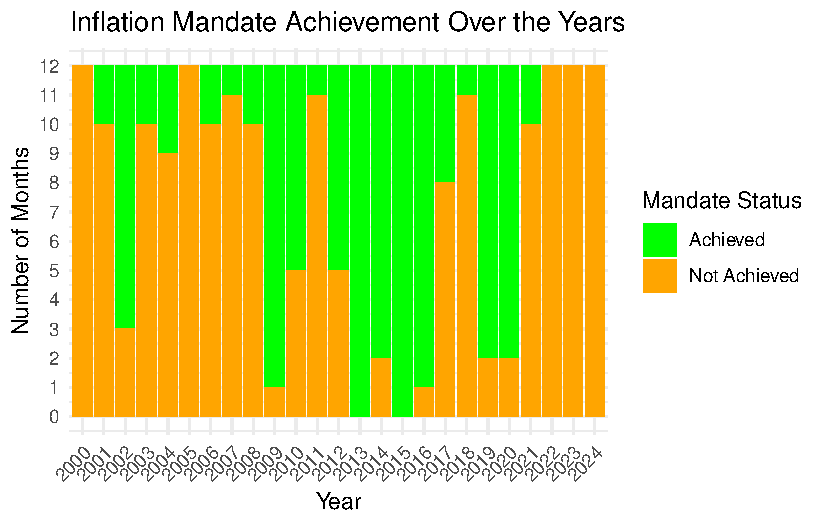
\includegraphics{Assignment2_Data608_Quarto_files/figure-pdf/unnamed-chunk-29-1.pdf}

\begin{Shaded}
\begin{Highlighting}[]
\FunctionTok{ggplot}\NormalTok{(unemp\_df, }\FunctionTok{aes}\NormalTok{(}\AttributeTok{x =} \FunctionTok{factor}\NormalTok{(Year), }\AttributeTok{fill =}\NormalTok{ unemp\_criteria)) }\SpecialCharTok{+}
  \FunctionTok{geom\_bar}\NormalTok{(}\AttributeTok{position =} \StringTok{"stack"}\NormalTok{) }\SpecialCharTok{+}  
  \FunctionTok{scale\_fill\_manual}\NormalTok{(}\AttributeTok{values =} \FunctionTok{c}\NormalTok{(}\StringTok{"Achieved"} \OtherTok{=} \StringTok{"blue"}\NormalTok{, }\StringTok{"Not Achieved"} \OtherTok{=} \StringTok{"pink"}\NormalTok{)) }\SpecialCharTok{+}
  \FunctionTok{scale\_y\_continuous}\NormalTok{(}\AttributeTok{breaks =} \FunctionTok{seq}\NormalTok{(}\DecValTok{0}\NormalTok{, }\DecValTok{12}\NormalTok{, }\AttributeTok{by =} \DecValTok{1}\NormalTok{)) }\SpecialCharTok{+}  \CommentTok{\# Ensure y{-}axis is in whole numbers (0 to 12)}
  \FunctionTok{labs}\NormalTok{(}\AttributeTok{title =} \StringTok{"Unemployment Mandate Achievement Over the Years"}\NormalTok{,}
       \AttributeTok{x =} \StringTok{"Year"}\NormalTok{,}
       \AttributeTok{y =} \StringTok{"Number of Months"}\NormalTok{,}
       \AttributeTok{fill =} \StringTok{"Mandate Status"}\NormalTok{) }\SpecialCharTok{+}
  \FunctionTok{theme\_minimal}\NormalTok{() }\SpecialCharTok{+}
  \FunctionTok{theme}\NormalTok{(}\AttributeTok{axis.text.x =} \FunctionTok{element\_text}\NormalTok{(}\AttributeTok{angle =} \DecValTok{45}\NormalTok{, }\AttributeTok{hjust =} \DecValTok{1}\NormalTok{))  }\CommentTok{\# Rotate x{-}axis labels}
\end{Highlighting}
\end{Shaded}

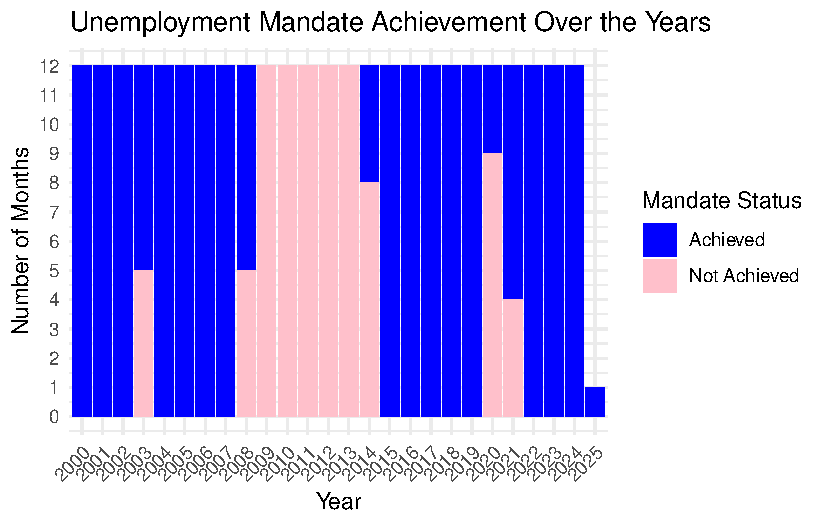
\includegraphics{Assignment2_Data608_Quarto_files/figure-pdf/unnamed-chunk-30-1.pdf}

\subsubsection{Ensure merged\_df is Properly
Structured}\label{ensure-merged_df-is-properly-structured}

\begin{Shaded}
\begin{Highlighting}[]
\CommentTok{\# Load necessary libraries}
\FunctionTok{library}\NormalTok{(dplyr)}
\FunctionTok{library}\NormalTok{(ggplot2)}
\FunctionTok{library}\NormalTok{(tidyr)}

\CommentTok{\# Ensure the Month column is a character type}
\NormalTok{merged\_df }\OtherTok{\textless{}{-}}\NormalTok{ merged\_df }\SpecialCharTok{\%\textgreater{}\%}
  \FunctionTok{mutate}\NormalTok{(}\AttributeTok{Month =} \FunctionTok{as.character}\NormalTok{(Month))}

\CommentTok{\# Convert to long format for better visualization}
\NormalTok{long\_df }\OtherTok{\textless{}{-}}\NormalTok{ merged\_df }\SpecialCharTok{\%\textgreater{}\%}
  \FunctionTok{pivot\_longer}\NormalTok{(}\AttributeTok{cols =} \FunctionTok{c}\NormalTok{(inflation\_criteria, unemp\_criteria),}
               \AttributeTok{names\_to =} \StringTok{"Mandate"}\NormalTok{,}
               \AttributeTok{values\_to =} \StringTok{"Status"}\NormalTok{)}

\CommentTok{\# Rename "Mandate" column for clarity}
\NormalTok{long\_df }\OtherTok{\textless{}{-}}\NormalTok{ long\_df }\SpecialCharTok{\%\textgreater{}\%}
  \FunctionTok{mutate}\NormalTok{(}\AttributeTok{Mandate =} \FunctionTok{ifelse}\NormalTok{(Mandate }\SpecialCharTok{==} \StringTok{"inflation\_criteria"}\NormalTok{, }\StringTok{"Inflation Mandate"}\NormalTok{, }\StringTok{"Unemployment Mandate"}\NormalTok{))}
\end{Highlighting}
\end{Shaded}

\subsubsection{Create the Stacked Bar
Chart}\label{create-the-stacked-bar-chart}

\subsubsection{Now visualizing combined Inflation \& Unemployment
Mandate Achievements over the
years.}\label{now-visualizing-combined-inflation-unemployment-mandate-achievements-over-the-years.}

\begin{Shaded}
\begin{Highlighting}[]
\FunctionTok{library}\NormalTok{(dplyr)}
\FunctionTok{library}\NormalTok{(ggplot2)}

\CommentTok{\# Ensure Year is numeric}
\NormalTok{long\_df}\SpecialCharTok{$}\NormalTok{Year }\OtherTok{\textless{}{-}} \FunctionTok{as.numeric}\NormalTok{(long\_df}\SpecialCharTok{$}\NormalTok{Year)}

\CommentTok{\# Count unique months per year (avoid double{-}counting Inflation \& Unemployment)}
\NormalTok{aggregated\_df }\OtherTok{\textless{}{-}}\NormalTok{ long\_df }\SpecialCharTok{\%\textgreater{}\%}
  \FunctionTok{group\_by}\NormalTok{(Year, Month, status) }\SpecialCharTok{\%\textgreater{}\%}
  \FunctionTok{summarise}\NormalTok{(}\AttributeTok{count =} \FunctionTok{n}\NormalTok{(), }\AttributeTok{.groups =} \StringTok{"drop"}\NormalTok{)  }\CommentTok{\# Count unique months per year}

\CommentTok{\# Define custom colors}
\NormalTok{colors }\OtherTok{\textless{}{-}} \FunctionTok{c}\NormalTok{(}\StringTok{"Yes"} \OtherTok{=} \StringTok{"green"}\NormalTok{,}
            \StringTok{"No"} \OtherTok{=} \StringTok{"red"}\NormalTok{,}
            \StringTok{"Partial Achieved"} \OtherTok{=} \StringTok{"orange"}\NormalTok{)}

\CommentTok{\# Create the stacked bar chart}
\FunctionTok{ggplot}\NormalTok{(aggregated\_df, }\FunctionTok{aes}\NormalTok{(}\AttributeTok{x =} \FunctionTok{factor}\NormalTok{(Year), }\AttributeTok{y =}\NormalTok{ count, }\AttributeTok{fill =}\NormalTok{ status)) }\SpecialCharTok{+}
  \FunctionTok{geom\_col}\NormalTok{(}\AttributeTok{position =} \StringTok{"stack"}\NormalTok{) }\SpecialCharTok{+}  \CommentTok{\# Use geom\_col for pre{-}aggregated data}
  \FunctionTok{scale\_fill\_manual}\NormalTok{(}\AttributeTok{values =}\NormalTok{ colors) }\SpecialCharTok{+}
  \FunctionTok{scale\_y\_continuous}\NormalTok{(}\AttributeTok{limits =} \FunctionTok{c}\NormalTok{(}\DecValTok{0}\NormalTok{, }\DecValTok{12}\NormalTok{), }\AttributeTok{breaks =} \DecValTok{0}\SpecialCharTok{:}\DecValTok{12}\NormalTok{) }\SpecialCharTok{+}  \CommentTok{\# Ensure Y{-}axis is 0{-}12 months}
  \FunctionTok{labs}\NormalTok{(}\AttributeTok{title =} \StringTok{"Mandate Achievement Over the Years (Inflation Target \textless{}= 2\%, Unemplyment Target \textless{}= 6\%)"}\NormalTok{,}
       \AttributeTok{x =} \StringTok{"Year"}\NormalTok{,}
       \AttributeTok{y =} \StringTok{"Number of Months Achieved"}\NormalTok{,}
       \AttributeTok{fill =} \StringTok{"Status"}\NormalTok{) }\SpecialCharTok{+}
  \FunctionTok{theme\_minimal}\NormalTok{() }\SpecialCharTok{+}
  \FunctionTok{theme}\NormalTok{(}\AttributeTok{axis.text.x =} \FunctionTok{element\_text}\NormalTok{(}\AttributeTok{angle =} \DecValTok{45}\NormalTok{, }\AttributeTok{hjust =} \DecValTok{1}\NormalTok{))  }\CommentTok{\# Rotate x{-}axis labels for readability}
\end{Highlighting}
\end{Shaded}

\begin{verbatim}
Warning: Removed 150 rows containing missing values or values outside the scale range
(`geom_col()`).
\end{verbatim}

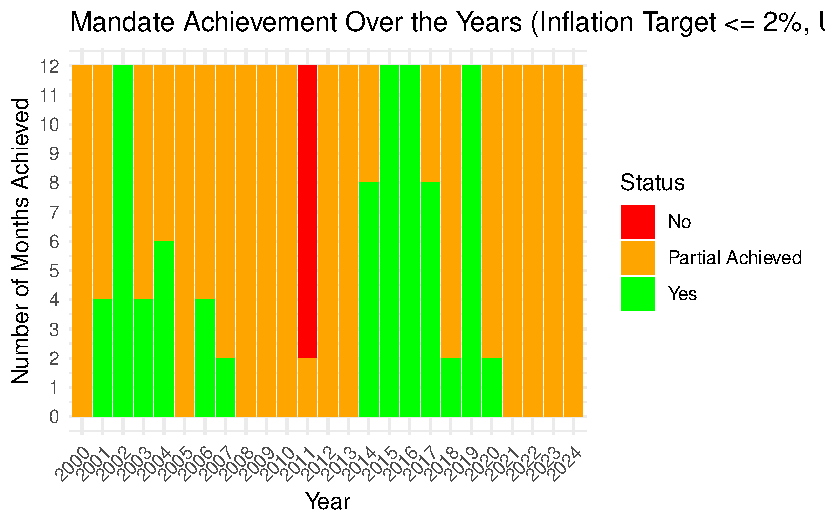
\includegraphics{Assignment2_Data608_Quarto_files/figure-pdf/unnamed-chunk-32-1.pdf}

\subsubsection{Interpreting the Chart: Has the Federal Reserve (FED)
Fulfilled Its
Mandate?}\label{interpreting-the-chart-has-the-federal-reserve-fed-fulfilled-its-mandate}

The stacked bar chart represents the FED's mandate achievement over time
(2000--2024), tracking whether it met its dual mandate of:

Stable Prices (Inflation Control) Maximum Employment The chart
categorizes each month per year into:

Yes -- Both inflation \& employment criteria were achieved. No --
Neither was achieved. Partial Achieved -- One was achieved, the other
was not.



\end{document}
